% !TeX spellcheck = en_GB
% %%% ***************** CHAPTER INTRODUCTION ***************** %%%
\chapter{Introduction}
\label{ch:intro}
%%%%%%%%% INTRODUCTION %%%%%%%%%%%%%%
Global warming is predicted to cause an increased frequency of extreme weather events and heat waves, droughts, heavy rains or extremely high winds \citep{hansen_warmer_2014}. Weather and climate extremes can have serious effects on human society and infrastructure, as well as on ecosystems and wildlife. Severe weather events are mostly in the focus of media reports with respect to global warming \citep{meehl_introduction_2000}. Understanding and predicting the impact of extreme weather events is one of the grand challenges of current climate research \citep{stocker_working_2013,field_summary_2014}.
\par\medskip
\noindent
This work focuses on the extreme weather event during Christmas 2016, and the snowfall measurements and model forecasts taken at the measurement site Haukeliseter in Southern Norway. The 2016 extreme Christmas storm, named 'Urd' by the Norwegian Meteorological Institute (Met-Norway), and had a large impact on Eastern, Southern, and Western Norway \citep{olsen_ekstremvaerrapport._2017}. Storms with high wind speed and precipitation amount are expected to occur approximately every five years. The financial costs associated with the 2016 Christmas storm are estimated to about 180 million Norwegian kroner. 'Urd' led to major traffic problems for cars, trains, ferries and air planes. Most mountain crossings were kept closed during Christmas 2016 \citep{olsen_ekstremvaerrapport._2017}. An increase in temperature and therefore a change of frozen to liquid precipitation followed an increase in avalanche danger. In addition, 40 emergency power stations failed during the extreme event affecting around 70.000 households (\Cref{fig:news}).
%a power blackout of around 70.000 households where 40 emergency power stations failed during the extreme weather (\Cref{fig:news}). 
Since people are affected by extreme weather it is important to accurately measure and forecast severe storms. The use of accurate observations will lead to better performing weather forecast models, which rely heavily on observations \citep{joos_influence_2012}. 
%%% images from Twitter and news %%%%%%%%%%%%%%%%%%%%%%%%%%%%%%%%%%%%%
% !TeX spellcheck = en_GB
\begin{figure}[t!]
	\centering
	\begin{subfigure}[b]{0.49\textwidth}
		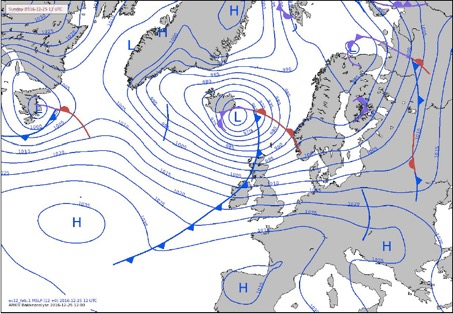
\includegraphics[width=\textwidth]{./fig_introduction/Ana_2512_12UTC.jpg}
		\caption{}\label{fig:ana_YR}
	\end{subfigure}
\hfill
	\begin{subfigure}[b]{0.49\textwidth}
		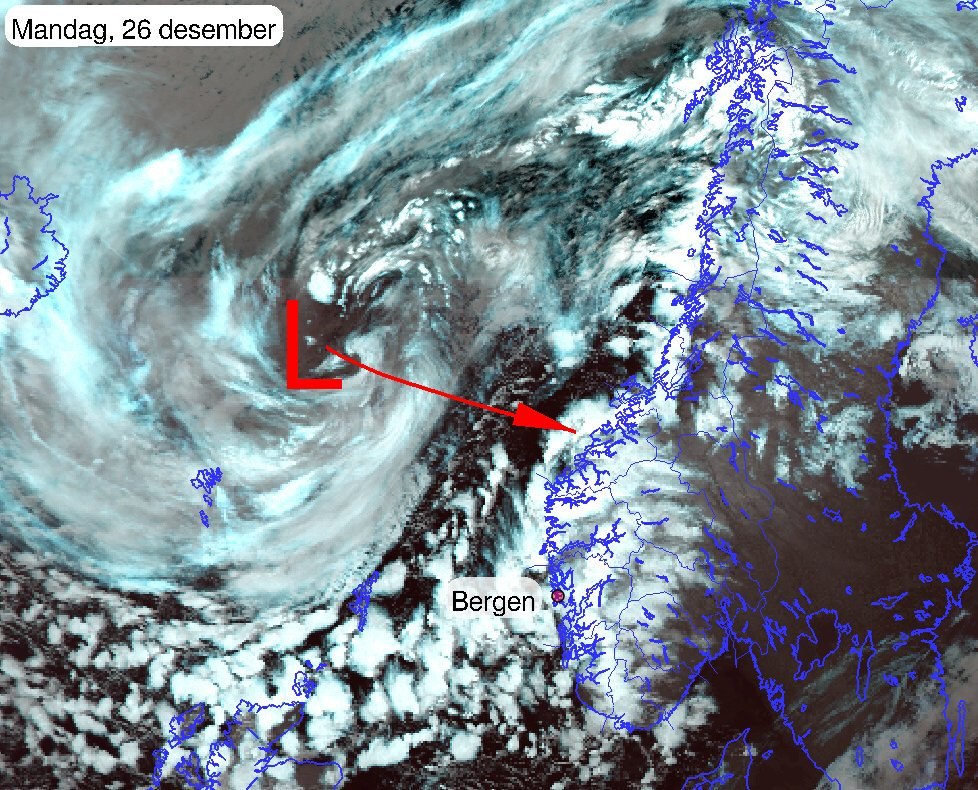
\includegraphics[trim={0cm 3.8cm 0cm 0cm},clip, width=\textwidth]{./fig_introduction/Twitter_26122016_0934AM.jpeg}
		\caption{}\label{fig:meteorologene_2612}	
	\end{subfigure}
	\begin{subfigure}[b]{0.49\textwidth}
		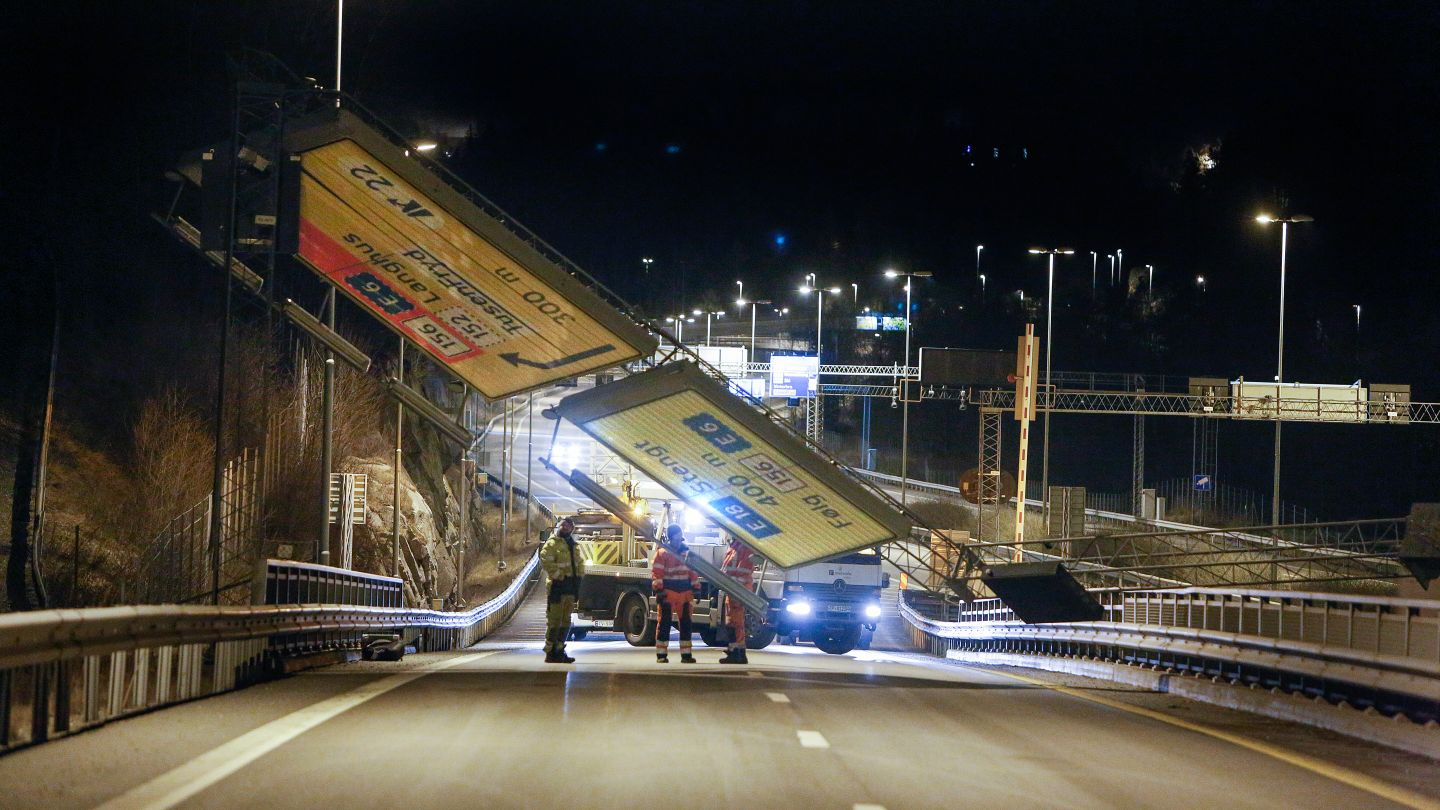
\includegraphics[width=\textwidth]{./fig_introduction/street_sign_2512.jpg}
		\caption{}\label{fig:street_sign}
	\end{subfigure}
\hfill
	\begin{subfigure}[b]{0.49\textwidth}
		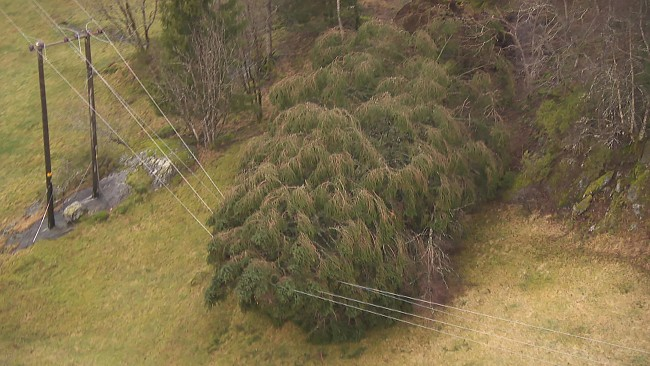
\includegraphics[width=\textwidth]{./fig_introduction/tree_nrk_2812.jpg}
		\caption{}\label{fig:tree_elec}
	\end{subfigure}
\caption{Weather situation during the extreme Christmas storm and impact on the infrastructure. In \protect\subref{fig:ana_YR}: Weather situation Sunday \SI{25}{\dec} at \SI{12}{\UTC} from the extreme weather report on Urd \citep{olsen_ekstremvaerrapport._2017}.
	\protect\subref{fig:meteorologene_2612}: Tweet from \cite{meteorologene_her_2016} on \SI{26}{\dec} at 9:34 am: Here comes \#Urd! The low pressure centre will hit M{\o}re og Romsdal, but the strongest wind comes south of Stad. \#S{\o}rNorge.
    \protect\subref{fig:street_sign} and \protect\subref{fig:tree_elec} show the consequences related to the high wind speeds during Christmas 2016.
	\protect\subref{fig:street_sign}: This traffic sign, ten meter long and four meter high was blown down during the storm, \citep{ruud_tonn_2016}.
	\protect\subref{fig:tree_elec}: Trouble maker: The extreme weather during Christmas created problems for the local infrastructure. \num{80.000} households were without electricity during the storm, \citep{farestveit_80.000_2016}.} \label{fig:news}
\end{figure}
%%%%%%%%%%%%%%%%%%%%%%%%%%%%%%%%%%%%%%%%%%%%%%%%%%%%%%%%%%%%%%%%%%%%%%%%%%
\par\medskip
\noindent
Since winter 2010, Haukeliseter has been a WMO measuring station with single and double fence precipitation instruments. In the winter of 2016/2017, three additional state of the art radar and snowflake microphysical instruments were deployed, which will be used to estimate the vertical profile of snow water content in the atmosphere. \citet{joos_influence_2012} showed in a sensitivity study of the microphysical scheme in a regional model for storm development, whether or not the location of the precipitation is correctly simulated.
%that when sensitivity studies on a regional model is applied, the storm development depends on whether or not the placement of the precipitation is correct in the simulated storm. 
Key was the precipitation profile, which determines which determines the vertical profile of latent heating. Latent heating leads to potential vorticity generation or destruction followed by a storm amplification or decrease, respectively. Vertical pointing radar reflectivity measurements are rare but can be an improvement to understand the microphysical structure in storms. Radar reflectivities were measured using the \SI{24}{\giga\hertz} Micro Rain Radar (MRR) at Haukeliseter. For this thesis, snowflake characteristics were estimated using a Multi-Angle Snowflake Camera \citep[MASC;][]{garrett_fall_2012} and a Precipitation Imaging Package \citep[PIP;][]{newman_presenting_2009}. 
%With the aid of the modified CloudSat snow particle model algorithm and the snowflake properties, as well as reflectivity profiles, the amount of snowfall in the atmosphere can then be determined. 
An optimal-estimation retrieval algorithm was developed that could estimate  snowfall rates consistent with each MRR, MASC, and PIP measurement. This method of estimating snowfall is much like the study from \citet{cooper_variational_2017} for Barrow, Alaska. The main difference between the studies of \citet{cooper_variational_2017} and this thesis here is that a \SI{24}{\giga\hertz} MRR is used instead of a \SI{94}{\giga\hertz} Ka-band ARM (The Atmospheric Radiation Measurement) zenith radar.
Additionally, the double fence measurements %should help to estimate vertically derived snowfall on the ground.
will provide a boundary condition to ensure that retrieved surface snowfall accumulations are close to the truth. Such agreement will in turn provide confidence in the retrieved snow water contents in the vertical column.
\\
The Meteorological Cooperation on Operational Numerical Weather Prediction (MetCoOp) Ensemble Prediction forecast (MEPS) has been operational at Met-Norway, since 2016. The ensemble prediction system uses the previous deterministic AROME-MetCoOp, a version of the Mèteo-France Applications of Research to Operations at MEsoscale (AROME). In addition to the deterministic forecast, nine perturbed ensemble members are initialised in MEPS. The newly developed ensemble prediction systems from Met-Norway is used to analyse the extreme winter storm during Christmas 2016. 
\\
The thesis is investigating in the thesis if the ensemble prediction system is able to forecast the variation of an extreme winter event such as 'Urd' and if the forecast model is able to predict large scale phenomena as well as local frozen precipitation. Furthermore, the use of an ensemble prediction system will give the possibility to compare the variation of snowfall precipitation at the surface and in the vertical. Observations will help to compare MEPS model forecast to examine the following research questions: 
Does the regional model cover local affects associated with the topography surrounding the measurement site?
Are large scale synoptic phenomena be resolved by MEPS?
How well does the model predict the surface snowfall at the Haukeliseter measurement site? \textcolor{red}{Is there a difference between estimated surface accumulation for different optimal estimation assumptions? }
\\
\\
The thesis is structured as following: The next section provides the background for the motivation of this thesis.
\Cref{ch:Methods} gives an overview of the measurement site Haukeliseter and its instrumentation, followed by the methodology on the optimal estimation retrieval as well as a description of the regional model MEPS, data transformation and the statistical analysis is presented in \Cref{sec:data_proc}.
The 2016 extreme Christmas event is analysed in \Cref{ch:weather_ana}. \Cref{ch:Res} will show the comparison between the double fence gauge measurement and the retrieved snowfall amount at the surface, analyse if large scale phenomena were predicted at Haukeliseter, and discuss overestimation of surface precipitation amount as well as the wind and snowfall related orographic influence.
%results and the discussion on large scale effects, surface snowfall accumulation and local wind influence at Haukeliseter. 
The final chapter summarises the results and gives an outloock for research.
%%%%%%%%%%%%%%%%%%%%%%%%%%%%%%%%%%%%%%%%%%%%%%%%%%%%%%%%%%%%	


\section{Background}
It has long been known that measuring precipitation, especially in the form of snow, is difficult. Winter precipitation measurement show biases of more than \SI{100}{\percent} between different gauge observation networks and different regions \citep{kochendorfer_analysis_2017}. The local climate changes from station to station leading to different habit and size of frozen aggregates. Measurement uncertainties can be caused by the instrument itself, which varies with wind speed, gauge wind shielding, shape, size, phase, and fall velocity in hydrometeors \citep{kochendorfer_analysis_2017,wolff_derivation_2015}. 
Uncertainties in precipitation measurements under windy conditions can affect water balance calculation and the calibration of remote sensing algorithms \citep{wolff_derivation_2015}. 
\\
Precipitation observations are important for hydrological, climate and weather research, as more than one-sixth of the world's population receives water from glaciers and seasonal snow packs \citep{barnett_potential_2005}.
\\
Since winds have an influence on frozen precipitation, a WMO (World Meteorological Organization) precipitation analysis between 1987 and 1993 recommended, that the double-fence inter-comparison reference should be used as a reference for snow measurements \citep{goodison_wmo_1998}. An adjustment for unshielded and single-shielded precipitation gauges followed in 2010. The adjustment transfer function, for single fence gauges, represents a capture efficiency as a function of air temperature and wind speed to delimit the error of measured snowfall \citep{kochendorfer_analysis_2017,wolff_derivation_2015}.
\par\medskip
\noindent
% Estimates of snowfall from radar reflectivities are non-unique. 
% %Nearly identical snowfall rates for given radar reflectivity signatures can be generated from various combinations of snowflake microphysical properties and particle fall velocity.
% This means, a given reflectivity can yield very different estimates of snowfall depending upon the precise microphysical assumptions used in the retrieval scheme.
% %This can lead for individual events to an error in retrieval uncertainties of \num{100}--\SI{200}{\percent} \citep{wood_estimation_2011}. 
% \citet{kulie_utilizing_2009}, for example, used the CloudSat Cloud Profiling Radar (CPR) reflectivities to estimate the global precipitation rate of dry snowfall through one year. They found that snowfall estimates critically depend on assumed snowfall particle size distribution, shape, and radar reflection. 
% %These studies suggest that snowfall estimates resulting only from radar reflections are ambiguous. Numerous different combinations of snowflake microphysical properties and snow particle falling rates can yield to nearly identical surface snowfall rates for a given reflectivity profile. 
% They concluded, that the use of traditional Ze-S relationships can lead to large differences when comparing snowfall events with different microphysics.
% \\
% %Based on observations of particle size distribution, fall velocity, snowflake habit, and a modified version of the optimal estimation CloudSat snowfall algorithm followed an average difference reduction to \SI{18}{\percent} of snowfall estimates, when compared to a National Weather Service measurement in Barrow, Alaska \citep{cooper_variational_2017}.
% Subsequent studies have tried to incorporate scene dependent microphysical information into the retrieval scheme.  \citet{wood_estimation_2011} embedded particle size distribution (PSD) - temperature relationship information into the CloudSat operational snowfall retrieval scheme to help reduce retrieval non-uniqueness. \citet{cooper_variational_2017} used in-situ estimates of snowflake PSD and habit from ground-based instrumentation to explore snowfall retrieval performance at Barrow, Alaska. They found reasonable agreement within \SI{20}{\percent} of nearby snow gauge measurements.
The quantitative estimation of snowfall at the global scale from spaceborne measurements has occurred only recently. Initial retrieval approaches were based on passive microwave measurements \citep{skofronick-jackson_physical_2004,noh_development_2006}. But since these passive measurements can only assess total integrated snow water path for a given column, such efforts were unable to provide much information on the vertical profiles of snow water. 
The launch of the CloudSat \SI{94}{\giga\hertz} Cloud Profiling Radar (CPR) in 2006, however, provided the first opportunity to examine such vertical structure at a global scale. Several studies, such as \citet{matrosov_modeling_2007} and \citet{kulie_utilizing_2009}, have shown that the CPR can be used to estimate snofall rate but that estimated snowfall values depend heavily upon assumed snowflake microphysical properties. So, for a given radar reflectivity, we can get large differences in estimated snow rate depending upon retrieval assumptions such as snowflake habit and particle size distribution (PSD).
%
%\citet{wood_microphysical_2015} showed that a refinement of the CloudSat snowfall retrieval algorithm can be performed by using snowflake models. This study was based on data from the Canadian CloudSat-CALIPSO Validation Project \citep[C3VP,][]{hudak_canadian_2006}, where they concentrated on cold season clouds and precipitation.
For the operational CloudSat snowfall retrieval scheme (2C-SNOW-PROFILE), \citet{wood_microphysical_2015} developed snowflake particle models based upon video snow disdrometer observations from the Canadian CloudSat-CALIPSO Validation Project \citep[C3VP,][]{hudak_canadian_2006}. Scattering properties for these snow particle models were based upon the Discrete Dipole Approximation (DDA) method. It was hoped that the use of realistic snow properties in the retrievals would lead to reasonable estimates of snowfall in the retrieval. In addition, they derived an a priori relationship between particle size distribution parameters and temperature that they could use as an additional constraint for the snowfall scheme. Use of the flexible optimal-estimation retrieval framework allowed a means to develop a best estimate of snow properties that are consistent with both the CPR reflectivities and the a priori constraint. 
\\
%In an attempt to reduce the non-uniqueness of the problem, \citet{wood_microphysical_2015} used the a priori knowledge of snowfall microphysics and temperature (from ground-based observations) to refine the forward-model assumptions for the CloudSat snowfall retrieval scheme. 
%Results from this scheme showed a good agreement with reported values observed at meteorological measurement sites \textcolor{red}{references}. 
%\\
%Model estimates have proven, how useful the estimation retrieval can be to verify ground-based radar snowfall measurements \citep{norin_intercomparison_2015}.Although the retrieval has obviously been improved the estimation algorithm, a priori guess can still lead to uncertainties in the retrievals of up to \SIrange{140}{200}{\percent} \citep{wood_estimation_2011}. 
They have also been used to estimate snowfall in remote locations such as the Antarctic and Arctic \citep{palerme_how_2014,kulie_shallow_2016}, that in turn, have been used to evaluate the representation of snowfall in climate models \citep{palerme_evaluation_2017,christensen_arctic_2016}. Similarly, these estimates have been used to assess the performance of ground-based radar schemes such as those based upon the operational weather radar system in Sweden \citep{norin_intercomparison_2015}. Despite such progress, however, the CloudSat scheme can still lead to uncertainties in the retrievals of up to \SIrange{140}{200}{\percent} \citep{wood_estimation_2011} for individual storms.
\\
%\citet{cooper_variational_2017} developed a technique to combine MRR, MASC, and PiP information into a common retrieval framework. Specifically, estimates of snowflake microphysical properties from the MRR are used as the a priori term in the optimal-estimation retrieval scheme. The usage of either MASC/PiP or MRR fall-speed can show which a priori guess in the retrieval gives the more accurate retrieved snowfall rate at the ground. 
Again, these uncertainties arise from the large variance in snowflake microphysical  properties as observed in nature. In response, \citet{cooper_variational_2017} explored the use of in-situ, event specific  observations of snowflake microphysical properties to improve radar-based retrievals of snowfall.  This work was based upon observations from the Ka-band ARM Zenith Radar (KAZR) and Multi-Angle Snow Camera (MASC) deployed at the ARM Climate Facility Site at Barrow in Spring 2014. This ground-based \SI{35}{\giga\hertz} retrieval scheme was modified from the space-borne \SI{94}{\giga\hertz} CloudSat retrieval scheme developed by \citet{wood_estimation_2011}. But instead of using a temperature dependent a priori characterisation of PSD, \citeauthor{cooper_variational_2017} introduced the in-situ observations of particle size distribution through the a priori terms of the optimal-estimation framework. 
\\
%The difference between the retrieval and the snow gauge observations was \SI{-18}{\percent} when applied to data from Barrow, Alaska.\\
%\citet{cooper_variational_2017} also showed that the retrieval is sensitive to habit and fall speed. The installation of a MRR, MASC, and PIP should help to adjust the particle models for graupels and rimed particles which are often observed at Haukeliseter. 
%
Preliminary analyses suggest good performance for this retrieval scheme at Barrow. Estimates of snowfall from the \citet{cooper_variational_2017} approach differed by \SI{18}{\percent} relative to nearby National Weather Service snow gauge measurements for total accumulation over multiple snow events. However, given limited snowfall observed at Barrow during the MASC deployment, it was difficult to come to any definitive conclusions about retrieval performance. The NSF (National Science Foundation) funded field campaign with MRR, MASC, and PIP (Precipitation Imaging Package) deployment at Haukeliseter provides an ideal opportunity to further explore this retrieval approach. This study will continue continue to examine the sensitivity of retrieval surface snowfall rate to assumptions of habit, fall speed, and particle size distribution as in \citet{cooper_variational_2017}. But the work presented here will be different in that we also will examine the vertical profiles of snowfall through the atmospheric column.  
%%%%%%%%%%%%%%%%%%%%%%%%%%%%%%%%%%%%%%%%%%%%%%%%%%%%%%%%%%%%%%%%%%%%%%%%%%%%%%%%%%%%%%%%%%%%
\par\medskip
\noindent
With the increasing expansion of computational power, developments of high-resolution numerical weather forecasting models with $\le$\SI{4}{\km} scales can be able to represent small-scale phenomena, such as convective dynamics \citep{gowan_validation_2018}. This enhancement provides weather services the ability to improve short-term weather forecasts for convective events, which can seriously impact infrastructure and society \citep{muller_arome-metcoop:_2017}. 
Information on magnitudes and location of maximum temperature is of significant importance when warnings are published by meteorologcial services for severe weather events and for further use in downstream impact model, e.g. NVE's (Norwegian Water Resources and Energy Directorate) hydrological model for flooding and avalanche risk.
The ability to use high-resolution models is also followed by various challenges, such as physical parametrisation schemes, accurate representation of topography, and data assimilation of high-resolution data \citep{sun_convective-scale_2005}.
\\
The weather forecast in Scandinavia covers a wide range of phenomena and includes continental, maritime and polar conditions. Norway has a complicate coastline, gradients in land use, as well as complex topography, which can complicate local weather forecasting of temperature, wind and precipitation \citep{muller_arome-metcoop:_2017}. \citet{colle_1314_2005,garvert_1314_2005,schwartz_reproducing_2014}, for example, have shown, that simulations of orographic precipitation can be improved in mountainous terrain for horizontal grid spacing below \SI{4}{\km}. Uncertainties on a convective scale can lead to a rapid error growth \citep{lorenz_atmospheric_1969}, hence high-resolution ensemble prediction makes it possible to estimate the forecast uncertainty by performing several model runs, each with different initial conditions. %\citep{gowan_validation_2018}
\par\medskip
\noindent
The Christmas storm in 2016, might not have led to the same damages as some of the extreme weather events of recent years. As people and infrastructure are affected by extreme weather, it is necessary to further improve the accuracy of snow-ground observations to better verify numerical weather forecasts, hydrological and climate models \citep{joos_influence_2012}. Changes in snow pack characteristics after extreme rain on snow events can lead to severe avalanches \citep{stimberis_glide_2011} and to the formation of thick layers of ice in the snow pack or on ground \citep{putkonen_rain--snow_2003,hansen_climate_2011}.

%%%%%%%%%%%%%%%%%%%%%%%%%%%%%%%%%%%%%%%%%%%%%%%%%%%%%%%%%%%%

% \section{Descripition of this study}
% The purpose of this study is to apply an optimal-estimation snowfall retrieval on ground based measurements to estimate the surface accumulation and vertical snow water content for an extreme event during Christmas 2016. These will later be used to compare to \SI{48}{\hour} MEPS model forecasts to see if the model was able to predict synoptical features and precipitation related to the extreme event 'Urd' in 2016. 
% \\
% \\
% This method of estimating snowfall is much like the study from \citet{cooper_variational_2017}. The main difference between the studies at Barrow, Alaska and this study is that a \SI{24}{\giga\hertz} MRR is used instead of a \SI{94}{\giga\hertz} Ka-band ARM zenith radar, and PSD and fall speed is estimated from MASC, PIP images and Doppler velocities, respectively.
% \\
% The comparison of the surface MEPS forecasts is similar to \citet{muller_arome-metcoop:_2017}. They presented the performance of the previous operational model at Met-Norway, AROME-MetCoOp, to the global forecast system ECMWF. Case studies were provided to demonstrate the ability of the deterministic model to capture extreme precipitation and wind events. 
% \\
% The thesis is structured as following: \Cref{ch:Methods} will give an overview of the measurement site Haukeliseter and its instrumentation, followed by the methodology on the optimal estimation retrieval as well a description of the regional model MEPS. The application to the data will be presented to compare the forecast system to the observations. The synoptics of the extreme Christmas storm in 2016 is analysed in \Cref{ch:weather_ana}. \Cref{ch:Res} will show the results and the discussion on large scale effects, surface snowfall accumulation and local wind influence  at Haukeliseter. The final chapter summarises the results and findings and suggests future research questions.